\documentclass[10pt,border=1pt]{standalone}
\usepackage[T1]{fontenc}
\usepackage{mathpazo}
\usepackage{amsmath,amssymb}
\usepackage{xcolor}
\usepackage{pgfplots}
\pgfplotsset{compat=1.18}
\usetikzlibrary{shapes.geometric,positioning,arrows.meta,calc}
\definecolor{okorange}{HTML}{E69F00}
\definecolor{oksky}{HTML}{56B4E9}
\definecolor{okgreen}{HTML}{009E73}
\definecolor{okblue}{HTML}{0072B2}
\definecolor{okverm}{HTML}{D55E00}
\definecolor{okpurple}{HTML}{CC79A7}
\colorlet{accent}{okverm}
\pgfplotsset{
  safenest/.style={
    tick label style={font=\footnotesize},
    label style={font=\small},
    title style={font=\small, align=left},
    legend style={font=\footnotesize, draw=none, fill=none, cells={anchor=west}},
    grid style={black!12, line width=0.3pt},
    axis line style={black!70, line width=0.4pt},
    tick style={black!70, line width=0.4pt},
    axis lines*=left,
  },
}
\newlength{\figwidth}
\tikzset{every node/.append style={execute at begin node={\hyphenpenalty=10000\exhyphenpenalty=10000\relax}}}
\setlength{\figwidth}{18.47cm}
\begin{document}
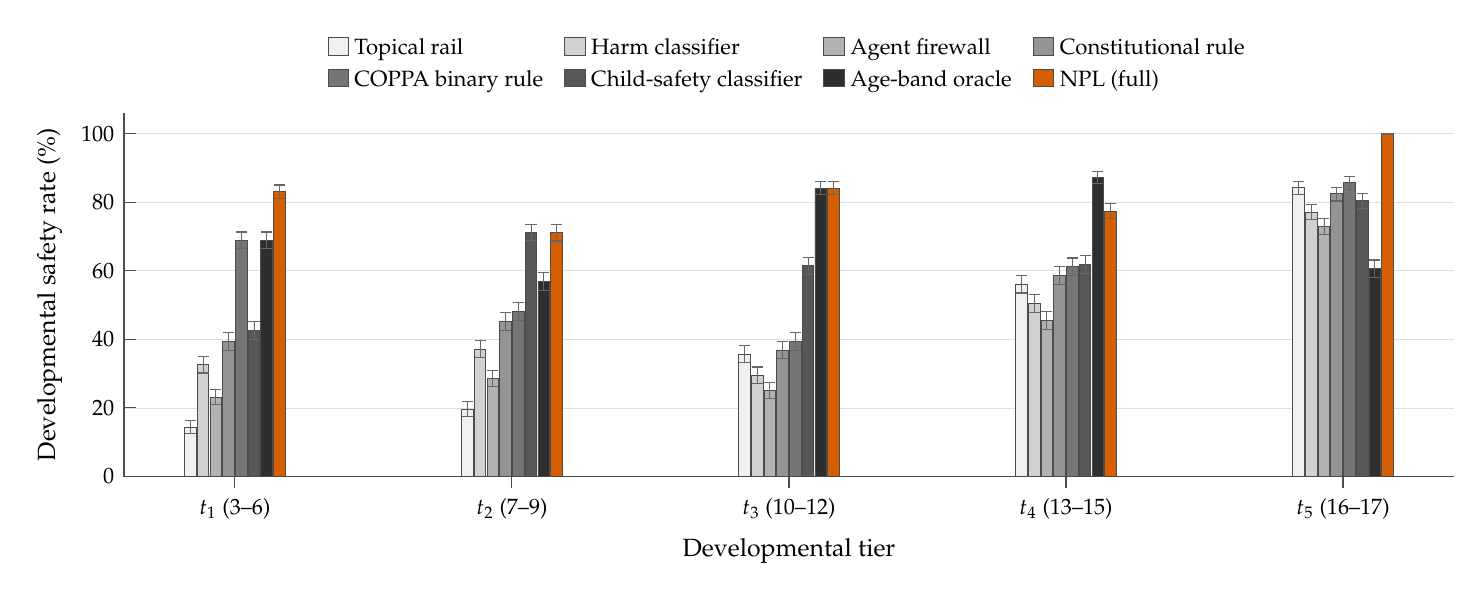
\begin{tikzpicture}
\begin{axis}[safenest, width=\figwidth, height=62mm,
  ybar=0.4pt, bar width=4.2pt, enlarge x limits=0.10, ymin=0, ymax=106,
  ytick={0,20,40,60,80,100},
  xtick={1,2,3,4,5}, xticklabels={$t_1$ (3--6),$t_2$ (7--9),$t_3$ (10--12),$t_4$ (13--15),$t_5$ (16--17)},
  xlabel={Developmental tier}, ylabel={Developmental safety rate (\%)},
  ymajorgrids,
  legend style={at={(0.5,1.03)}, anchor=south, legend columns=4,
                /tikz/every even column/.append style={column sep=1.2ex}},
  legend image code/.code={\draw[#1] (0cm,-0.08cm) rectangle (0.26cm,0.14cm);},
]
\addplot[ybar, fill=black!6, draw=black!70, line width=0.3pt,
  error bars/.cd, y dir=both, y explicit,
  error bar style={line width=0.3pt, black!60}]
  coordinates {(1,14.3) -= (0,1.74) += (0,1.93) (2,19.6) -= (0,1.99) += (0,2.16) (3,35.6) -= (0,2.47) += (0,2.54) (4,56.1) -= (0,2.61) += (0,2.58) (5,84.3) -= (0,2.00) += (0,1.81)};
\addlegendentry{Topical rail}
\addplot[ybar, fill=black!18, draw=black!70, line width=0.3pt,
  error bars/.cd, y dir=both, y explicit,
  error bar style={line width=0.3pt, black!60}]
  coordinates {(1,32.6) -= (0,2.41) += (0,2.50) (2,37.1) -= (0,2.49) += (0,2.56) (3,29.5) -= (0,2.33) += (0,2.44) (4,50.4) -= (0,2.62) += (0,2.61) (5,77.1) -= (0,2.27) += (0,2.13)};
\addlegendentry{Harm classifier}
\addplot[ybar, fill=black!30, draw=black!70, line width=0.3pt,
  error bars/.cd, y dir=both, y explicit,
  error bar style={line width=0.3pt, black!60}]
  coordinates {(1,23.1) -= (0,2.13) += (0,2.28) (2,28.5) -= (0,2.30) += (0,2.42) (3,25.0) -= (0,2.20) += (0,2.33) (4,45.4) -= (0,2.59) += (0,2.62) (5,73.0) -= (0,2.39) += (0,2.26)};
\addlegendentry{Agent firewall}
\addplot[ybar, fill=black!42, draw=black!70, line width=0.3pt,
  error bars/.cd, y dir=both, y explicit,
  error bar style={line width=0.3pt, black!60}]
  coordinates {(1,39.4) -= (0,2.53) += (0,2.58) (2,45.1) -= (0,2.59) += (0,2.62) (3,36.9) -= (0,2.49) += (0,2.56) (4,58.6) -= (0,2.60) += (0,2.55) (5,82.4) -= (0,2.08) += (0,1.90)};
\addlegendentry{Constitutional rule}
\addplot[ybar, fill=black!54, draw=black!70, line width=0.3pt,
  error bars/.cd, y dir=both, y explicit,
  error bar style={line width=0.3pt, black!60}]
  coordinates {(1,68.9) -= (0,2.47) += (0,2.37) (2,48.1) -= (0,2.61) += (0,2.62) (3,39.3) -= (0,2.53) += (0,2.58) (4,61.2) -= (0,2.58) += (0,2.52) (5,85.7) -= (0,1.93) += (0,1.74)};
\addlegendentry{COPPA binary rule}
\addplot[ybar, fill=black!66, draw=black!70, line width=0.3pt,
  error bars/.cd, y dir=both, y explicit,
  error bar style={line width=0.3pt, black!60}]
  coordinates {(1,42.5) -= (0,2.57) += (0,2.61) (2,71.2) -= (0,2.43) += (0,2.31) (3,61.4) -= (0,2.58) += (0,2.52) (4,61.8) -= (0,2.57) += (0,2.51) (5,80.4) -= (0,2.16) += (0,2.00)};
\addlegendentry{Child-safety classifier}
\addplot[ybar, fill=black!82, draw=black!70, line width=0.3pt,
  error bars/.cd, y dir=both, y explicit,
  error bar style={line width=0.3pt, black!60}]
  coordinates {(1,68.9) -= (0,2.47) += (0,2.37) (2,56.8) -= (0,2.61) += (0,2.57) (3,84.1) -= (0,2.01) += (0,1.82) (4,87.2) -= (0,1.85) += (0,1.65) (5,60.6) -= (0,2.59) += (0,2.53)};
\addlegendentry{Age-band oracle}
\addplot[ybar, fill=accent, draw=black!70, line width=0.3pt,
  error bars/.cd, y dir=both, y explicit,
  error bar style={line width=0.3pt, black!60}]
  coordinates {(1,83.1) -= (0,2.05) += (0,1.87) (2,71.1) -= (0,2.43) += (0,2.32) (3,84.1) -= (0,2.01) += (0,1.82) (4,77.4) -= (0,2.27) += (0,2.12) (5,100.0) -= (0,0.27) += (0,-0.00)};
\addlegendentry{NPL (full)}
\end{axis}
\end{tikzpicture}
\end{document}
